\documentclass{article}

\usepackage{fancyhdr}
\usepackage{extramarks}
\usepackage{amsmath}
\usepackage{amsthm}
\usepackage{amsfonts}
\usepackage{tikz}
\usepackage[plain]{algorithm}
\usepackage{algpseudocode}
\usepackage[figuresonly, nomarkers]{endfloat}

\usetikzlibrary{automata,positioning}

% Custom operators

\newcommand{\argmin}[1]{\underset{#1}{\operatorname{arg}\,\operatorname{min}}\;}
\newcommand{\argmax}[1]{\underset{#1}{\operatorname{arg}\,\operatorname{max}}\;}

% Endfloat settings

\renewcommand{\efloatseparator}{\mbox{}}

%
% Basic Document Settings
%

\topmargin=-0.45in
\evensidemargin=0in
\oddsidemargin=0in
\textwidth=6.5in
\textheight=9.0in
\headsep=0.25in

\linespread{1.1}

\pagestyle{fancy}
\lhead{\hmwkAuthorName}
\chead{\hmwkClass\ (\hmwkClassInstructor): \hmwkTitle}
\rhead{\firstxmark}
\lfoot{\lastxmark}
\cfoot{\thepage}

\renewcommand\headrulewidth{0.4pt}
\renewcommand\footrulewidth{0.4pt}

\setlength\parindent{0pt}

%
% Create Problem Sections
%

\newcommand{\enterProblemHeader}[1]{
    \nobreak\extramarks{}{Problem \arabic{#1} continued on next page\ldots}\nobreak{}
    \nobreak\extramarks{Problem \arabic{#1} (continued)}{Problem \arabic{#1} continued on next page\ldots}\nobreak{}
}

\newcommand{\exitProblemHeader}[1]{
    \nobreak\extramarks{Problem \arabic{#1} (continued)}{Problem \arabic{#1} continued on next page\ldots}\nobreak{}
    \stepcounter{#1}
    \nobreak\extramarks{Problem \arabic{#1}}{}\nobreak{}
}

\setcounter{secnumdepth}{0}
\newcounter{partCounter}
\newcounter{homeworkProblemCounter}
\setcounter{homeworkProblemCounter}{1}
\nobreak\extramarks{Problem \arabic{homeworkProblemCounter}}{}\nobreak{}

%
% Homework Problem Environment
%
% This environment takes an optional argument. When given, it will adjust the
% problem counter. This is useful for when the problems given for your
% assignment aren't sequential. See the last 3 problems of this template for an
% example.
%
\newenvironment{homeworkProblem}[1][-1]{
    \ifnum#1>0
        \setcounter{homeworkProblemCounter}{#1}
    \fi
    \section{Problem \arabic{homeworkProblemCounter}}
    \setcounter{partCounter}{1}
    \enterProblemHeader{homeworkProblemCounter}
}{
    \exitProblemHeader{homeworkProblemCounter}
}

%
% Homework Details
%   - Title
%   - Due date
%   - Class
%   - Section/Time
%   - Instructor
%   - Author
%

\newcommand{\hmwkTitle}{Written Homework\ \#10}
\newcommand{\hmwkDueDate}{17 November 2015}
\newcommand{\hmwkClass}{EECS 440}
\newcommand{\hmwkClassInstructor}{Professor Ray Soumya}
\newcommand{\hmwkAuthorName}{Michael Schaffer}

%
% Title Page
%

\title{
    \vspace{2in}
    \textmd{\textbf{\hmwkClass:\ \hmwkTitle}}\\
    \normalsize\vspace{0.1in}\small{Due\ on\ \hmwkDueDate}\\
    \vspace{0.1in}\large{\textit{\hmwkClassInstructor}}
    \vspace{3in}
}

\author{\textbf{\hmwkAuthorName}}
\date{}

\renewcommand{\part}[1]{\textbf{\large Part \Alph{partCounter}}\stepcounter{partCounter}\\}

%
% Various Helper Commands
%

% Useful for algorithms
\newcommand{\alg}[1]{\textsc{\bfseries \footnotesize #1}}

% For derivatives
\newcommand{\deriv}[1]{\frac{\mathrm{d}}{\mathrm{d}x} (#1)}

% For partial derivatives
\newcommand{\pderiv}[2]{\frac{\partial}{\partial #1} (#2)}

% Integral dx
\newcommand{\dx}{\mathrm{d}x}

% Alias for the Solution section header
\newcommand{\solution}{\textbf{\large Solution}}

% Probability commands: Expectation, Variance, Covariance, Bias
\newcommand{\E}{\mathrm{E}}
\newcommand{\Var}{\mathrm{Var}}
\newcommand{\Cov}{\mathrm{Cov}}
\newcommand{\Bias}{\mathrm{Bias}}

% Figures

\begin{figure}
	\centering
	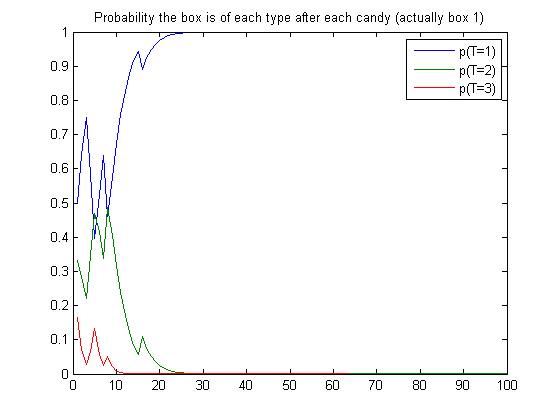
\includegraphics[width=0.7\linewidth]{q1box1}
	\caption{caption}
	\label{fig:q1box1}
\end{figure}

\begin{figure}
	\centering
	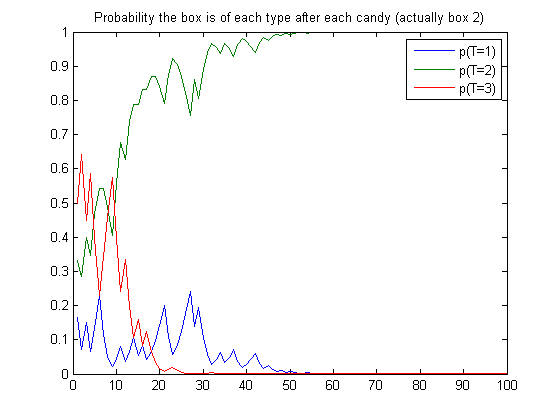
\includegraphics[width=0.7\linewidth]{q1box2}
	\caption{caption}
	\label{fig:q1box2}
\end{figure}

\begin{figure}
	\centering
	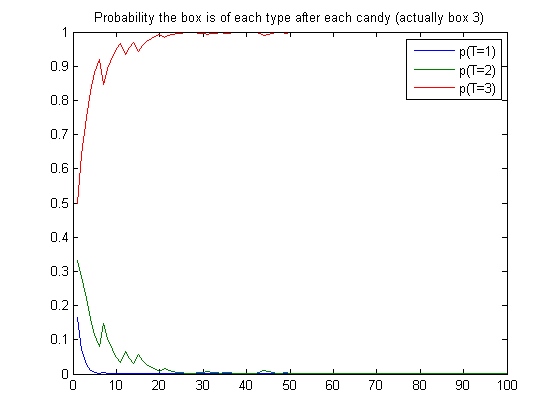
\includegraphics[width=0.7\linewidth]{q1box3}
	\caption{caption}
	\label{fig:q1box3}
\end{figure}

\begin{figure}
	\centering
	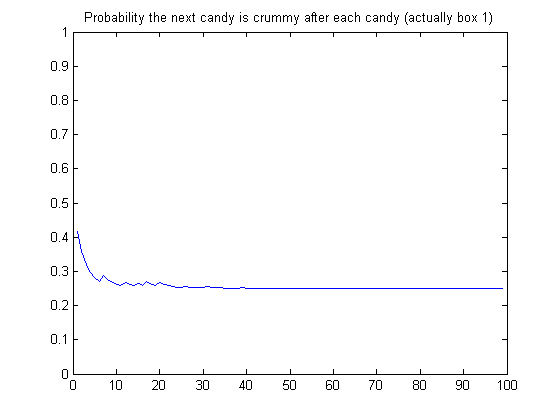
\includegraphics[width=0.7\linewidth]{q2box1}
	\caption{caption}
	\label{fig:q2box1}
\end{figure}

\begin{figure}
	\centering
	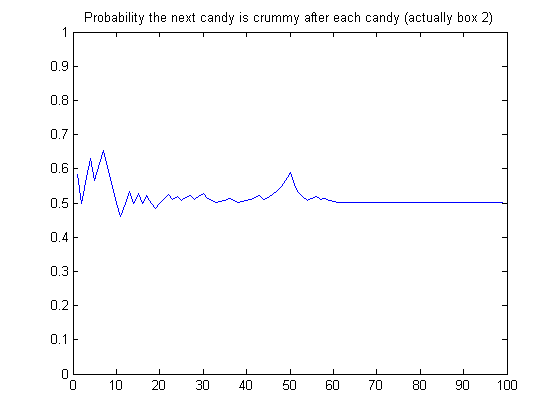
\includegraphics[width=0.7\linewidth]{q2box2}
	\caption{caption}
	\label{fig:q2box2}
\end{figure}

\begin{figure}
	\centering
	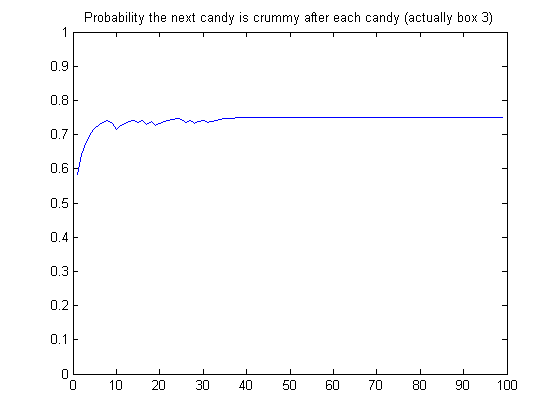
\includegraphics[width=0.7\linewidth]{q2box3}
	\caption{caption}
	\label{fig:q2box3}
\end{figure}

\begin{figure}
	\centering
	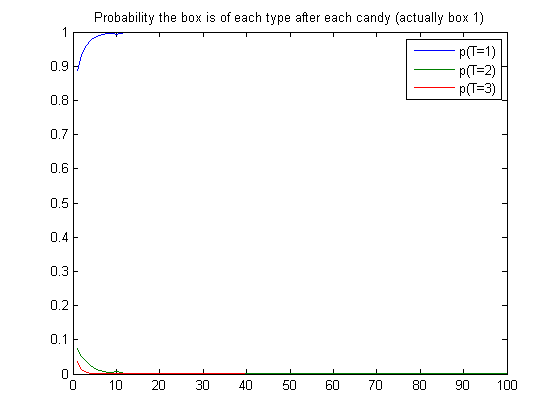
\includegraphics[width=0.7\linewidth]{q3box1}
	\caption{caption}
	\label{fig:q3box1}
\end{figure}

\begin{figure}
	\centering
	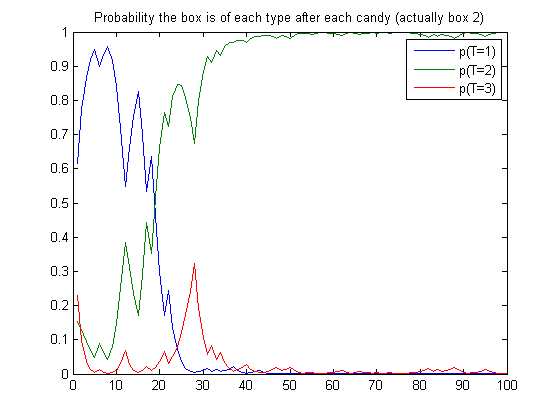
\includegraphics[width=0.7\linewidth]{q3box2}
	\caption{caption}
	\label{fig:q3box2}
\end{figure}

\begin{figure}
	\centering
	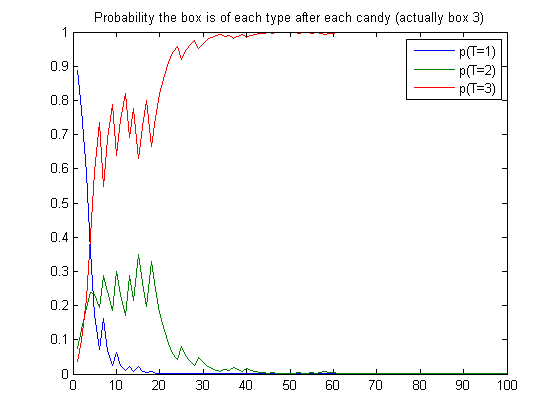
\includegraphics[width=0.7\linewidth]{q3box3}
	\caption{caption}
	\label{fig:q3box3}
\end{figure}

\begin{figure}
	\centering
	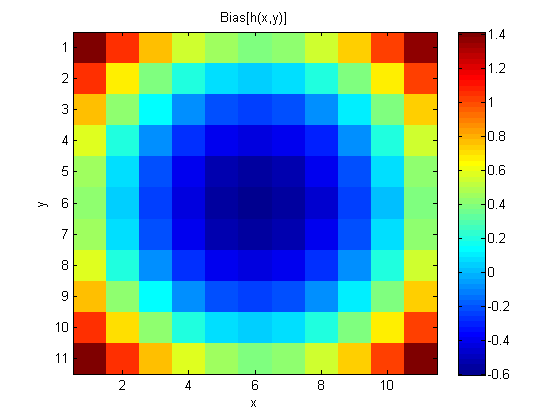
\includegraphics[width=0.7\linewidth]{bias}
	\caption{caption}
	\label{fig:bias}
\end{figure}

\begin{figure}
	\centering
	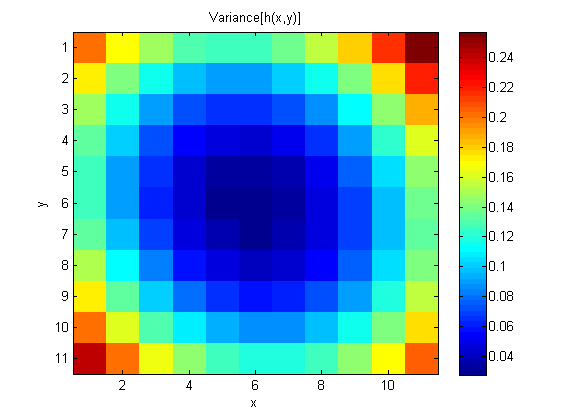
\includegraphics[width=0.7\linewidth]{variance}
	\caption{caption}
	\label{fig:variance}
\end{figure}

% Main document

\begin{document}

\maketitle

\pagebreak

\begin{homeworkProblem}
	
	 The Bayesian Candy Factory makes a Halloween Candy Box that contains a mix of yummy
	 (Y) and crummy (C) candy. You know that each Box is one of three types: 1. 75\% Y and 25\% C,
	 2. 50\% Y and 50\% C and 3. 25\% Y and 75\% C. You open a Box and start munching candies. Let
	 the $i^{th}$ candy you munch be denoted by $c_i$. Answer the following questions using MATLAB, R or
	 any other math package. Generate one Box with 100 candies for each type, and assume a fixed
	 order of munching.
	 
	 \begin{enumerate}
	 	\item
	 	For each Box, plot $Pr(T=i|c_1,…,c_N)$ on a graph where $T$ represents a type
	 	and $N$ ranges from 1 to 100. (You should have three graphs and each graph will have three
	 	curves.)
	 	
	 	\item
	 	For each Box, plot $Pr(c_{N+1}=C|c_1,…,c_N)$ where $N$ ranges from 1 to 99.
	 	
	 	\item
	 	Suppose you are an optimist, and before opening a Box you believe that each Box has 75\% Y (type 1)
	 	with probability 0.8 and the probability of the other two types is 0.1 each. Redo part (1) taking
	 	this belief into account. Briefly explain the implications of your results.
	 	
	 \end{enumerate}

    \textbf{Solution}
    
    \begin{enumerate}
    	\item
    	See figures \ref{fig:q1box1}, \ref{fig:q1box2}, and \ref{fig:q1box3}.
    	
    	\item
    	See figures \ref{fig:q2box1}, \ref{fig:q2box2}, and \ref{fig:q2box3}.
    	
    	\item
    	See figures \ref{fig:q3box1}, \ref{fig:q3box2}, and \ref{fig:q3box3}. These results show that in the long run, the initial prior probability only influences the amount of time it takes to converge on the correct result, not what that result actually is. This finding does not necessarily apply to higher-dimensional hypothesis spaces with more local optima.
    	
    \end{enumerate}

\end{homeworkProblem}

\pagebreak

\begin{homeworkProblem}
	
	When estimating parameters for a Boolean attribute $f$ in a na{\"i}ve Bayes model, it is observed
	that $f$ is true in $k$ out of $n$ positive examples. Further, there is a Dirichlet prior on the parameter
	representing the probability of $f$ given a positive example, with hyper-parameters $a$ and $b$. Show
	that the MAP estimate of the parameter’s value is equivalent to an $m$-estimate with specific
	values of $m$ and $p$. In this way show that $m$-estimates act as Bayesian prior knowledge in na{\"i}ve
	Bayes. The Dirichlet distribution over $0 \leq \theta \leq 1$ is given by: $D(\theta;a,b)=[(a-1)! (b-1)! / (a+b-1)!] \theta
	(a-1) (1- \theta)(b-1)$ where $a$, $b$ are positive integers greater than 1 and are parameters of the
	distribution.
     
    \textbf{Solution}
    
    Let $Y$ be the parameter representing the probability of $f$ given a positive example.
    
    For the MAP estimate:
    
    \[ MAP = \argmax{y} Pr(X=x|Y=y)Pr(Y=y) \]
    \[ Pr(X=x|Y=y) = y \]
    \[ Pr(Y=y) = D(y;a,b) = [(a-1)! (b-1)! / (a+b-1)!] y (a-1) (1-y) (b-1) \]
    \[ MAP = \argmax{y} [(a-1)! (b-1)! / (a+b-1)!] (a-1) (b-1) y^2 (1-y) \]
    \[ MAP = \argmax{y} y^2 (1-y) \]
    \[ \frac{d}{dy} y^2 (1-y) = 0 \]
    \[ 2y - 3y^2 = 0 \]
    \[ y = \{ 0, \frac{2}{3} \} \]
    \[ y = \frac{2}{3} \]
    
    For the m-estimate:
    
    \[ y = \frac{k + mp}{n + m} = \frac{2}{3} \]
    \[ 2n+2m = 3k+3mp \]
    \[ m(2-3p) = 3k-2n \]
    
    This shows that you can always choose values of m and p that will get the same estimate as the MAP estimate.

\end{homeworkProblem}

\pagebreak

\begin{homeworkProblem}
	
	 Consider a regression problem with examples described by 2 continuous attributes, $x$ and $y$.
	 Each example is sampled according to the uniform distribution on $(-1,1)^2$ and labeled with
	 $f(x,y)=1-x^2-y^2$. A learner’s hypothesis class is $h(x,y)=ax+by+c$.
	 
	 \begin{enumerate}
	 	\item
	 	Calculate its bias and variance as a function of x and y if the learner sees an arbitrarily large training sample.
	 	
	 	\item
	 	Using MATLAB, find the (x,y) with the largest bias and the (x,y) with the largest variance for samples
	 	of size 10. Can you intuitively justify your findings?
	 	
	 \end{enumerate}
	
	\textbf{Solution}
	
	\begin{enumerate}
		\item
		Since the training sample is arbitrarily large, the distribution of resulting hypotheses will converge to the single least-squares hypothesis:
		
		\[ \argmin{a, b, c} \int_{-1}^1 \int_{-1}^1 (h(x,y) - f(x,y))^2 \,dx\,dy \]
		\[ = \argmin{a, b, c} \int_{-1}^1 \int_{-1}^1 ((ax+by+c) - (1-x^2-y^2))^2 \,dx\,dy \]
		\[ = \argmin{a, b, c} \int_{-1}^1 \int_{-1}^1 (x^2+y^2+ax+by+c-1)^2 \,dx\,dy \]
		\[ = \argmin{a, b, c} \int_{-1}^1 \frac{2}{3}(a^2+2(y^2+by+c-1))+2(y^2+by+c-1)^2+\frac{2}{5} \,dy \]
		\[ = \argmin{a, b, c} \frac{4}{3}a^2+\frac{4}{3}b^2+4c^2-\frac{8}{3}c+\frac{52}{45} \]
		\[ = \argmin{a} \frac{4}{3}a^2 + \argmin{b} \frac{4}{3}b^2 + \argmin{c} (4c^2-\frac{8}{3}c) + \frac{52}{45} \]
		\[a=0, b=0 \]
		\[ \frac{d}{dc} (4c^2-\frac{8}{3}c) = 0 \]
		\[ 8c - \frac{8}{3} = 0 \]
		\[ c = \frac{1}{3} \]
		\[ h(x,y) = \frac{1}{3} \]
		
		For the bias:
		
		\[ Bias[h(x,y)] = E[h(x,y)] - f(x,y) \]
		\[ Bias[h(x,y)] = \frac{1/3} - (1-x^2-y^2) \]
		\[ Bias[h(x,y)] = x^2 + y^2 - \frac{2}{3} \]
		
		For the variance:
		
		\[ Var[h(x,y)] = E[(h(x,y)-E[h(x,y)])^2] = E[(\frac{1}{3} - \frac{1}{3})^2] = 0 \]
		
		\item
		Figure \ref{fig:bias} shows the bias of $h(x,y)$, and figure \ref{fig:variance} shows the variance.
		
		The (x,y) coordinates with the largest bias are visually (-1,-1), (-1,1), (1,-1), and (1,1).
		
		The (x,y) coordinates with the largest variance are visually the same four.
		
		It makes intuitive sense that the bias is largest at the corners because they are the lowest points of f(x,y), and the bias depends negatively on f.
		
		It makes intuitive sense that the variance is largest at the corners because the linear regression hypotheses will generally get the slope somewhat wrong, making it more accurate for the center of the distribution of examples than for the outskirts.
		
	\end{enumerate}
    
\end{homeworkProblem}

\begin{homeworkProblem}
	
	Suppose a learner uses bootstrap resampling to construct a training sample $T$ from an initial
	sample $U$, of the same size as $U$. Show that, for a large enough $U$, the probability that some
	example from $U$ appears in $T$ is approximately 0.63.
	
	\textbf{Solution}

\end{homeworkProblem}

\end{document}
